\documentclass[12pt,a4paper]{article}
\usepackage[a4paper,top=2.54cm,bottom=2.54cm,left=3.17cm,right=3.17cm]{geometry}
\usepackage{fontspec}
\usepackage{xeCJK}
\usepackage{setspace}
\usepackage{fancyhdr}
\usepackage{amsmath,amssymb,bm}
\usepackage{graphicx,booktabs}
\usepackage{float}
\usepackage{placeins}
\usepackage{algorithm,algorithmic}
\usepackage{caption,subcaption}
\usepackage[super,square,numbers,sort&compress]{natbib}
\usepackage{xcolor,hyperref}

% Preferred university fonts: Times New Roman for English and numerals,
% Arial for sans serif text, Courier New for monospaced text, and SimSun
% (Songti) for any CJK glyphs. TeX Gyre and Fandol fonts are safe fallbacks.
\IfFontExistsTF{Times New Roman}
  {\setmainfont{Times New Roman}}
  {\setmainfont{TeX Gyre Termes}}
\IfFontExistsTF{Arial}
  {\setsansfont{Arial}}
  {\setsansfont{TeX Gyre Heros}}
\IfFontExistsTF{Courier New}
  {\setmonofont{Courier New}}
  {\setmonofont{TeX Gyre Cursor}}
\IfFontExistsTF{SimSun}
  {\setCJKmainfont{SimSun}}
  {\setCJKmainfont{FandolSong-Regular}}

\graphicspath{{figures/}}
\captionsetup{
  font={small,stretch=1.5},
  labelfont=bf
}
\hypersetup{
  pdftitle={Adaptive Variance-Stabilized Projected Gradient Descent for Low-Dose PET Image Preprocessing},
  pdfauthor={Undergraduate Candidate},
  colorlinks=true,
  linkcolor=black,
  citecolor=blue,
  urlcolor=blue
}
\onehalfspacing
\pagestyle{fancy}
\fancyhf{}
\fancyfoot[C]{\fontsize{7.5pt}{9pt}\selectfont\thepage}
\renewcommand{\headrulewidth}{0pt}
\renewcommand{\footrulewidth}{0pt}
\fancypagestyle{plain}{
  \fancyhf{}
  \fancyfoot[C]{\fontsize{7.5pt}{9pt}\selectfont\thepage}
  \renewcommand{\headrulewidth}{0pt}
  \renewcommand{\footrulewidth}{0pt}
}
\newcommand{\R}{\mathbb{R}}
\renewcommand{\refname}{References}
\newcommand{\ProposedPSNRFifty}{34.16}
\newcommand{\ProposedPSNRTwentyFive}{31.49}
\newcommand{\ProposedPSNRTen}{27.87}
\newcommand{\ProposedGainTwentyFive}{6.82}
\newcommand{\ProposedOverNLMTwentyFive}{0.85}
\newcommand{\ProposedIterFifty}{31}
\newcommand{\ProposedIterTwentyFive}{40}
\newcommand{\ProposedIterTen}{140}
\newcommand{\AdaptiveWeightPSNRLoss}{0.58}
\newcommand{\FixedStepPSNR}{31.95}
\newcommand{\FixedStepIterations}{140}
\newcommand{\FixedStepRuntimeRatio}{8.3}
\newcommand{\BestLambdaOne}{2}
\newcommand{\BestLambdaTwo}{0.5}
\newcommand{\BestSensitivityPSNR}{31.49}


\title{\textbf{Adaptive Variance-Stabilized Projected Gradient Descent\\
for Low-Dose PET Image Preprocessing}}
\author{Undergraduate Candidate\\
Biomedical and Computational Imaging Programme}
\date{}

\begin{document}
\pagenumbering{arabic}
\maketitle
\begin{abstract}
\normalsize
Low-count positron emission tomography (PET) is degraded by signal-dependent Poisson fluctuations, whereas indiscriminate smoothing can erase small lesions. This study proposes Adaptive VST-PGD, an image-preprocessing method that combines the Anscombe variance-stabilizing transform with non-negative, spatially adaptive first- and second-order regularization. The resulting objective is minimized by projected gradient descent using a Barzilai--Borwein spectral step and Armijo backtracking. Experiments on a reproducible $256\times256$ PET-like Shepp--Logan phantom compare the method with Gaussian filtering, non-local means, and total-variation gradient descent at 50\%, 25\%, and 10\% dose levels. Adaptive VST-PGD achieves the highest PSNR at all three levels (\ProposedPSNRFifty, \ProposedPSNRTwentyFive, and \ProposedPSNRTen{} dB, respectively). Ablation, convergence, and parameter-sensitivity analyses quantify the contributions of variance stabilization, adaptive weighting, and spectral step selection. These results establish an interpretable numerical baseline for low-dose PET preprocessing; clinical effectiveness remains to be validated on physical phantom and patient data.

\end{abstract}
\noindent\textbf{Keywords:} Low-dose PET, image preprocessing, Poisson noise,
Anscombe transform, projected gradient descent, adaptive regularization
\vspace{1em}

\section{Introduction}
Positron emission tomography (PET) maps radiotracer activity through coincident photon detection. Reducing injected activity or acquisition duration lowers the expected number of detected events and increases stochastic variation. A Poisson model remains a useful first approximation after common corrections and normalization, although reconstructed clinical images also contain spatial correlations and modelling errors \citep{shepp1982maximum,qi2006iterative}. Low-dose PET preprocessing must therefore suppress count-dependent fluctuations without biasing uptake values or erasing lesion boundaries.

Conventional Gaussian filtering does not account for signal-dependent statistics. Non-local means (NLM) exploits repeated patches, but patch similarity becomes unreliable under severe noise \citep{buades2005nonlocal}. Total variation (TV) preserves discontinuities but can introduce staircase artefacts \citep{rudin1992nonlinear}. This study addresses these limitations through a variance-stabilized objective that adapts first- and second-order regularization to local image structure.

The main contributions are: (i) a variance-stabilized formulation for low-count PET-like data; (ii) an edge-adaptive combination of first- and second-order penalties; (iii) a non-negative projected gradient solver with Barzilai--Borwein spectral steps and Armijo backtracking; and (iv) a reproducible evaluation including baseline comparison, convergence analysis, ablation, and parameter sensitivity. All reported numerical values are generated from the saved experiment outputs.

\section{Related Work}
PET reconstruction is commonly formulated from a Poisson likelihood, with expectation--maximization providing a seminal estimator \citep{shepp1982maximum}. Modern iterative reconstruction incorporates physical corrections and priors \citep{qi2006iterative}. Post-reconstruction denoising remains attractive when raw projection data are unavailable, but it cannot recover information absent from the acquisition.

The Anscombe transform maps a Poisson variable to an approximately unit-variance Gaussian variable \citep{anscombe1948transformation}. More accurate inverse formulae reduce low-count bias \citep{makitalo2011optimal}; nevertheless, the conventional algebraic inverse is retained here to match the defined experimental model. TV regularization formalizes edge-preserving smoothing \citep{rudin1992nonlinear}, while higher-order models mitigate piecewise-constant staircasing \citep{bredies2010total}. Spatial adaptation can interpolate between these behaviors using evidence from a pilot image.

Projected gradient descent enforces simple convex constraints \citep{bertsekas1999nonlinear}. Barzilai--Borwein steps approximate curvature from successive iterates at negligible memory cost \citep{barzilai1988two}, while Armijo backtracking provides a descent safeguard \citep{nocedal2006numerical}. Learned PET methods have also shown promise \citep{gong2019pet}, but variational baselines retain advantages in interpretability, reproducibility, and limited-data settings.

\section{Methodology}
\subsection{Low-Dose PET Noise Model}
Let $x\in\R_+^N$ denote the activity image and let $y$ denote the measured count image. The simplified observation model is
\begin{equation}
y_i\sim\operatorname{Poisson}(\alpha x_i+b_i),
\label{eq:poisson}
\end{equation}
where $\alpha$ represents dose or count scaling and $b_i$ represents background events. The simulation sets $b_i=0$ and uses count peaks of 60, 30, and 12 for the reported 50\%, 25\%, and 10\% dose levels.

\subsection{Anscombe Variance Stabilization}
The transformed observation is
\begin{equation}
z_i=2\sqrt{y_i+\frac{3}{8}},
\label{eq:anscombe}
\end{equation}
whose conditional variance is approximately one outside the extreme low-count regime. After optimization, the conventional algebraic inverse is applied:
\begin{equation}
\widehat{x}_i=\max\!\left\{(u_i/2)^2-3/8,0\right\}/\alpha.
\label{eq:inverse}
\end{equation}

\subsection{Adaptive First- and Second-Order Regularization}
Forward differences $D_x,D_y$ and second differences $D_{xx},D_{xy},D_{yy}$ use periodic boundaries. A robust edge scale $s$ is defined as the 90th percentile of $|\nabla z|$, and the spatial weight is
\begin{equation}
w_i=\exp\left[-\min\{|\nabla z_i|/s,4\}^2\right].
\label{eq:weight}
\end{equation}
The weight is close to one in flat regions, strengthening first-order suppression, while $(1-w)$ activates the second-order component near detected structures. The objective is
\begin{align}
E(u)=&\tfrac12\|u-z\|_2^2
+\lambda_1\sum_iw_i\sqrt{(D_xu_i)^2+(D_yu_i)^2+\epsilon^2}\nonumber\\
&+\lambda_2\sum_i(1-w_i)
\sqrt{(D_{xx}u_i)^2+2(D_{xy}u_i)^2+(D_{yy}u_i)^2+\epsilon^2}.
\label{eq:objective}
\end{align}
Writing $q_i$ and $r_i$ for the first- and second-order square-root terms, direct differentiation gives
\begin{align}
\nabla E(u)=&(u-z)+\lambda_1\left[
D_x^T\frac{wD_xu}{q}+D_y^T\frac{wD_yu}{q}\right]\nonumber\\
&+\lambda_2\left[
D_{xx}^T\frac{(1-w)D_{xx}u}{r}
+2D_{xy}^T\frac{(1-w)D_{xy}u}{r}
+D_{yy}^T\frac{(1-w)D_{yy}u}{r}\right].
\label{eq:gradient}
\end{align}

\subsection{Projected Gradient Descent Optimization}
Non-negativity is imposed through the projected update
\begin{equation}
u^{k+1}=\Pi_{\R_+^N}\!\left(u^k-\eta_k\nabla E(u^k)\right),
\label{eq:pgd}
\end{equation}
where projection is componentwise clipping. For $s_k=u^k-u^{k-1}$ and $v_k=g^k-g^{k-1}$, the Barzilai--Borwein proposal is
\begin{equation}
\eta_k^{\mathrm{BB}}=\operatorname{clip}\left(
\frac{s_k^Ts_k}{|s_k^Tv_k|+10^{-12}},10^{-4},0.2\right).
\label{eq:bb}
\end{equation}
Armijo backtracking halves this proposal until sufficient decrease is obtained. With fixed $w$ and $\epsilon>0$, Eq.~\eqref{eq:objective} is a smooth convex approximation over a closed convex feasible set. Under standard assumptions, backtracking ensures descent and accumulation points satisfy the projected first-order stationarity condition \citep{bertsekas1999nonlinear}. Small values of $\epsilon$ can nevertheless cause ill-conditioning, and the algebraic inverse remains biased in the extreme low-count regime.

\subsection{Proposed Adaptive VST-PGD Algorithm}
The complete optimization procedure is summarized in Algorithm~\ref{alg:method}. Starting from the variance-stabilized low-dose PET image, the proposed method iteratively minimizes the adaptive regularized objective using projected gradient descent with an Armijo-type step-size rule. The non-negativity projection guarantees physically meaningful PET intensities, while the inverse Anscombe transform maps the optimized image back to the original count domain.

\begin{algorithm}[H]
\caption{Adaptive VST-PGD for Low-Dose PET Image Preprocessing}
\label{alg:method}
\begin{algorithmic}[1]
\REQUIRE Low-dose image $y$, count scale $\alpha$, regularization parameters $\lambda_1,\lambda_2$, tolerance $\tau$
\STATE $z\gets2\sqrt{\alpha y+3/8}$; compute $w$ from Eq.~\eqref{eq:weight}; initialize $u^0\gets z$
\FOR{$k=0,1,\ldots,K-1$}
  \STATE Evaluate $E(u^k)$ and $g^k$ using Eqs.~\eqref{eq:objective}--\eqref{eq:gradient}
  \STATE Propose $\eta_k$ from Eq.~\eqref{eq:bb}, using $0.08$ at the initial iteration
  \REPEAT
    \STATE $u^{k+1}\gets\max(u^k-\eta_kg^k,0)$
    \STATE If the Armijo condition fails, set $\eta_k\gets\eta_k/2$
  \UNTIL{the decrease condition holds or 12 trials have been evaluated}
  \IF{$\|u^{k+1}-u^k\|_2/(\|u^k\|_2+10^{-12})<\tau$}
    \STATE \textbf{break}
  \ENDIF
\ENDFOR
\STATE \RETURN inverse transform from Eq.~\eqref{eq:inverse}
\end{algorithmic}
\end{algorithm}

The algorithm terminates when the relative change between two consecutive iterates falls below the tolerance threshold or when the maximum number of iterations is reached. This design preserves the interpretability of gradient-based optimization while improving robustness under low-count PET noise.

\FloatBarrier
\section{Experiments}
\subsection{Data Preparation}
A Shepp--Logan phantom was resized to $256\times256$ pixels and augmented with three small Gaussian hot lesions. Intensities were normalized to $[0,1]$. Independent Poisson draws with seed 20260627 used peak counts of 60, 30, and 12 to represent the 50\%, 25\%, and 10\% dose conditions, respectively.

\subsection{Baseline Methods}
Adaptive VST-PGD was compared with the unprocessed low-dose observation, Gaussian filtering, non-local means (NLM), and TV gradient descent (TV-GD). Gaussian filtering used a standard deviation of 1. NLM used $5\times5$ patches and a search distance of 6. TV-GD used $\lambda=0.08$ for 120 iterations. These methods provide representative linear, patch-based, and variational baselines.

\subsection{Evaluation Metrics}
PSNR, SSIM, RMSE, relative error (RE), and edge preservation index (EPI) were evaluated against ground truth. EPI is the cosine similarity between Sobel gradient vectors, so larger values indicate stronger gradient alignment. PSNR, SSIM, and EPI are maximized; RMSE and RE are minimized. Iteration counts are zero for non-iterative methods.

\subsection{Implementation Details}
Adaptive VST-PGD used $\lambda_1=2.0$, $\lambda_2=0.5$, $\epsilon=10^{-3}$, and at most 140 iterations. Barzilai--Borwein proposals were clipped to $[10^{-4},0.2]$, and Armijo backtracking used at most 12 trials per iteration. Runtime was measured with a monotonic wall clock. Tables and figures were generated programmatically from saved arrays and CSV files.

\section{Results and Discussion}
\subsection{Quantitative Comparison}
\begin{table}[tbp]
\centering
\caption{Measured performance across dose levels.}
\label{tab:metrics}
\setlength{\tabcolsep}{3pt}
\begin{tabular}{@{}llrrrrrrr@{}}\toprule
Dose & Method & PSNR & SSIM & RMSE & RE & EPI & Time (s) & Iter.\\ \midrule
50\% & Low-dose & 27.61 & 0.735 & 0.0416 & 0.172 & 0.959 & 0.0000 & 0 \\
50\% & Gaussian & 26.09 & 0.895 & 0.0496 & 0.204 & 0.935 & 0.0005 & 0 \\
50\% & NLM & 33.20 & 0.970 & 0.0219 & 0.090 & 0.992 & 0.0252 & 0 \\
50\% & TV-GD & 31.56 & 0.562 & 0.0264 & 0.109 & 0.991 & 0.0395 & 120 \\
50\% & Adaptive VST-PGD & 34.16 & 0.935 & 0.0196 & 0.081 & 0.992 & 0.0631 & 31 \\
25\% & Low-dose & 24.67 & 0.696 & 0.0584 & 0.241 & 0.922 & 0.0000 & 0 \\
25\% & Gaussian & 25.87 & 0.857 & 0.0509 & 0.210 & 0.928 & 0.0004 & 0 \\
25\% & NLM & 30.64 & 0.953 & 0.0294 & 0.121 & 0.986 & 0.0225 & 0 \\
25\% & TV-GD & 30.27 & 0.553 & 0.0307 & 0.126 & 0.986 & 0.0373 & 120 \\
25\% & Adaptive VST-PGD & 31.49 & 0.899 & 0.0266 & 0.110 & 0.985 & 0.0795 & 40 \\
10\% & Low-dose & 20.68 & 0.653 & 0.0925 & 0.381 & 0.824 & 0.0000 & 0 \\
10\% & Gaussian & 25.10 & 0.788 & 0.0556 & 0.229 & 0.905 & 0.0005 & 0 \\
10\% & NLM & 27.48 & 0.909 & 0.0423 & 0.174 & 0.972 & 0.0239 & 0 \\
10\% & TV-GD & 26.94 & 0.467 & 0.0450 & 0.185 & 0.958 & 0.0379 & 120 \\
10\% & Adaptive VST-PGD & 27.87 & 0.839 & 0.0404 & 0.166 & 0.966 & 0.2972 & 140 \\
\bottomrule\end{tabular}
\end{table}
Adaptive VST-PGD achieved the highest PSNR at every dose. At 25\% dose, it improved the low-dose input by \ProposedGainTwentyFive{} dB and exceeded NLM by \ProposedOverNLMTwentyFive{} dB. NLM achieved the highest SSIM, indicating that pixelwise fidelity and perceptual structural similarity favor different estimates. TV-GD attained high PSNR and EPI but substantially lower SSIM. Figure~\ref{fig:bars} summarizes PSNR and SSIM at 25\% dose.
\begin{figure}[tbp]
\centering
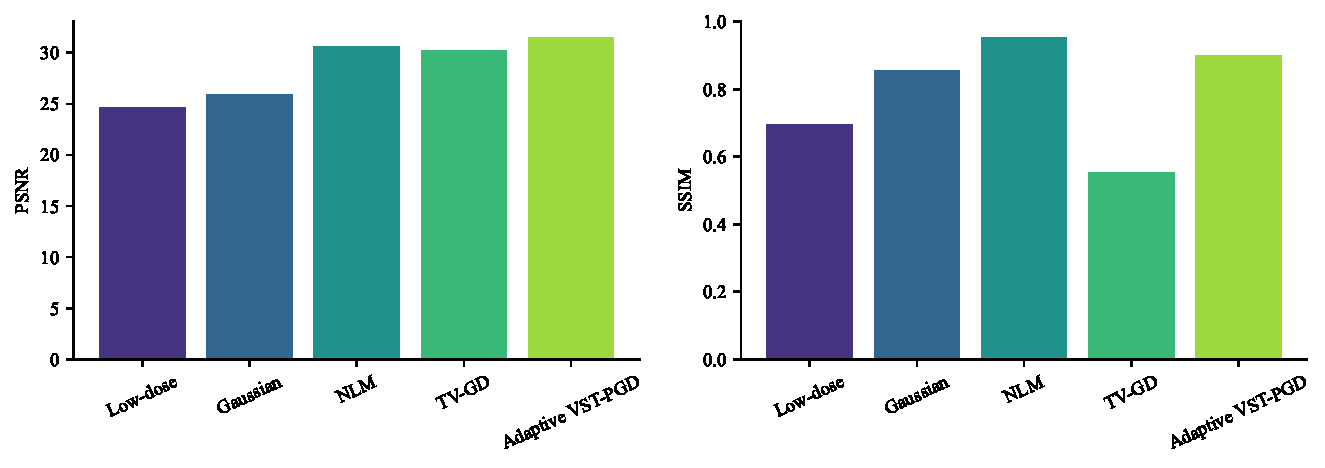
\includegraphics[width=.82\textwidth]{metric_bars.pdf}
\caption{PSNR and SSIM comparison at 25\% dose, generated from the measured results.}
\label{fig:bars}
\end{figure}

\subsection{Visual Comparison}
Figures~\ref{fig:comparison}--\ref{fig:zoom} compare reconstructed appearance and absolute errors at 25\% dose. The line profile in Fig.~\ref{fig:profile} provides a complementary assessment of local activity preservation through a hot lesion.
\begin{figure}[tbp]
\centering
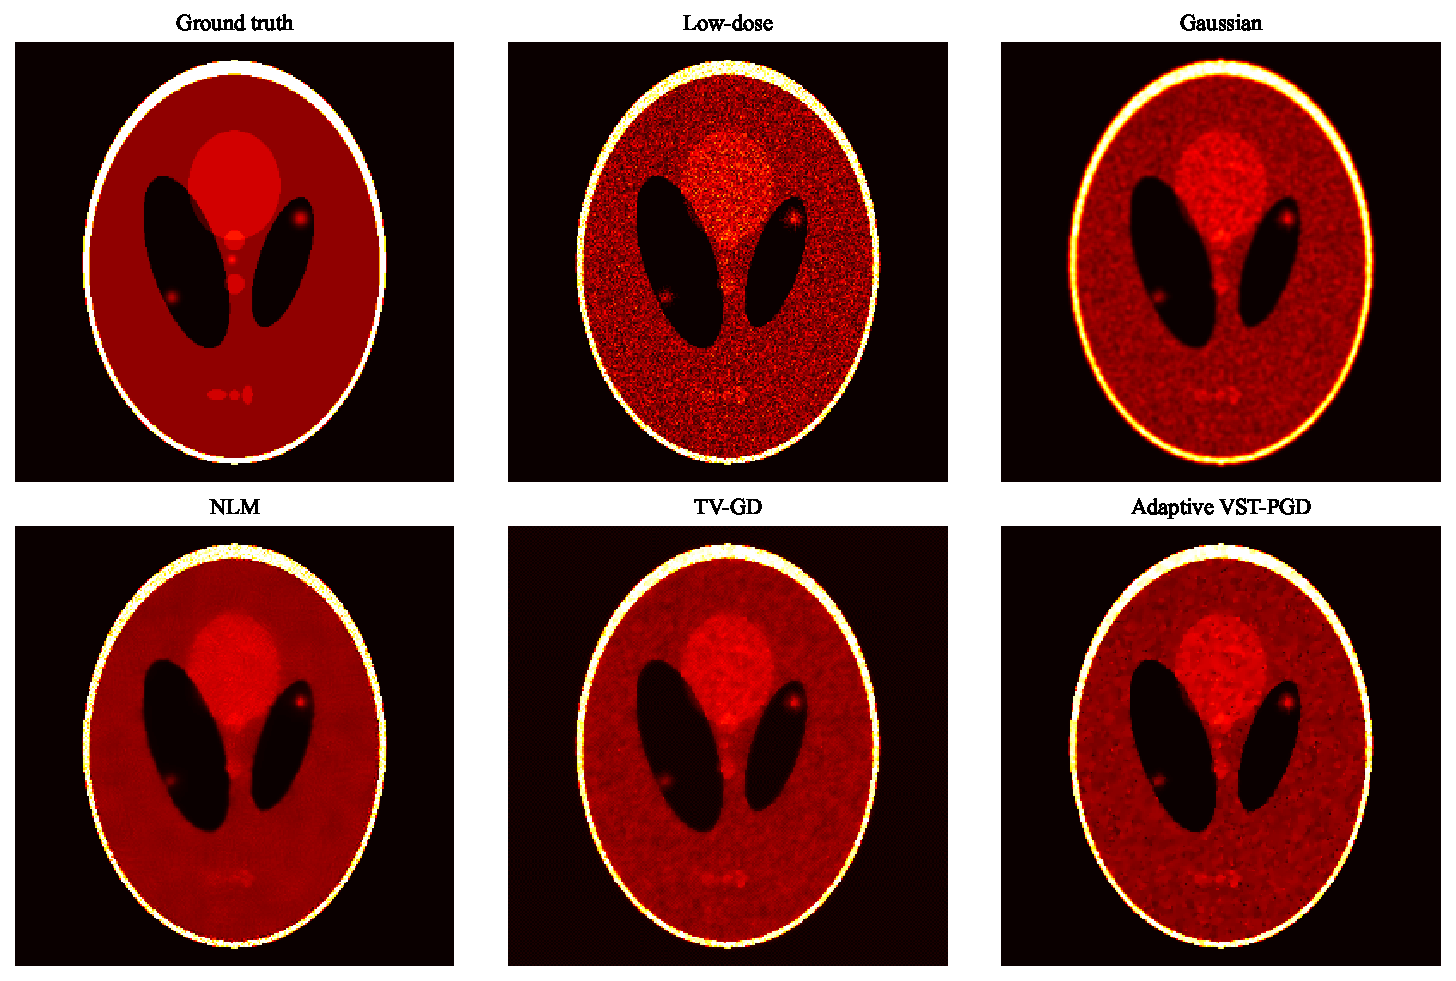
\includegraphics[width=.94\textwidth]{method_comparison.pdf}
\caption{Ground truth and preprocessing results at 25\% dose.}
\label{fig:comparison}
\end{figure}
\begin{figure}[tbp]
\centering
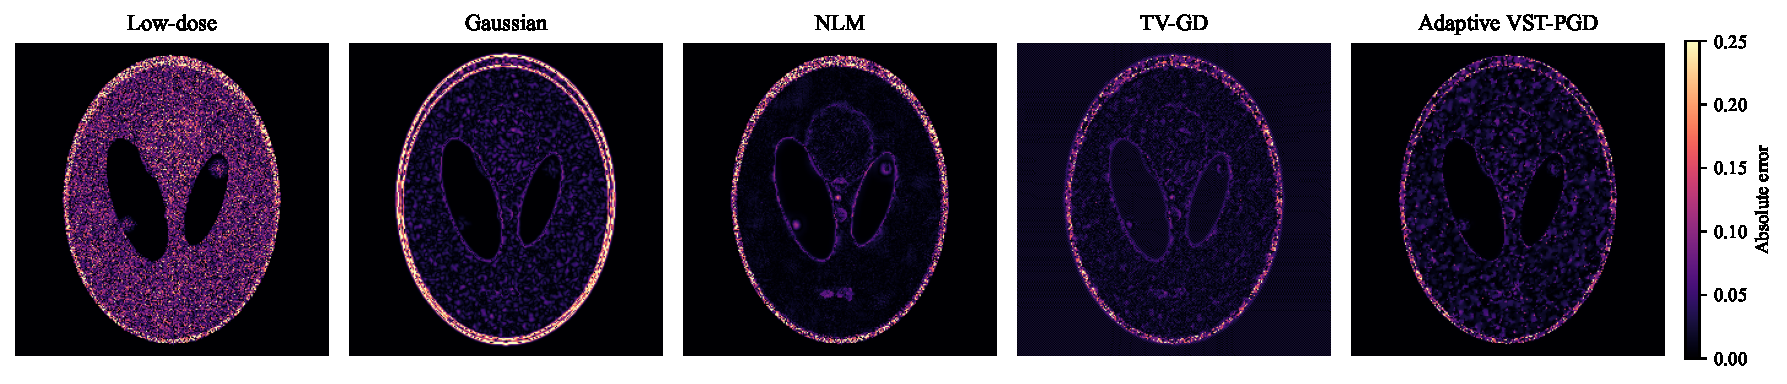
\includegraphics[width=.94\textwidth]{error_maps.pdf}
\caption{Absolute error maps at 25\% dose, displayed on a common scale.}
\label{fig:error}
\end{figure}
\begin{figure}[tbp]
\centering
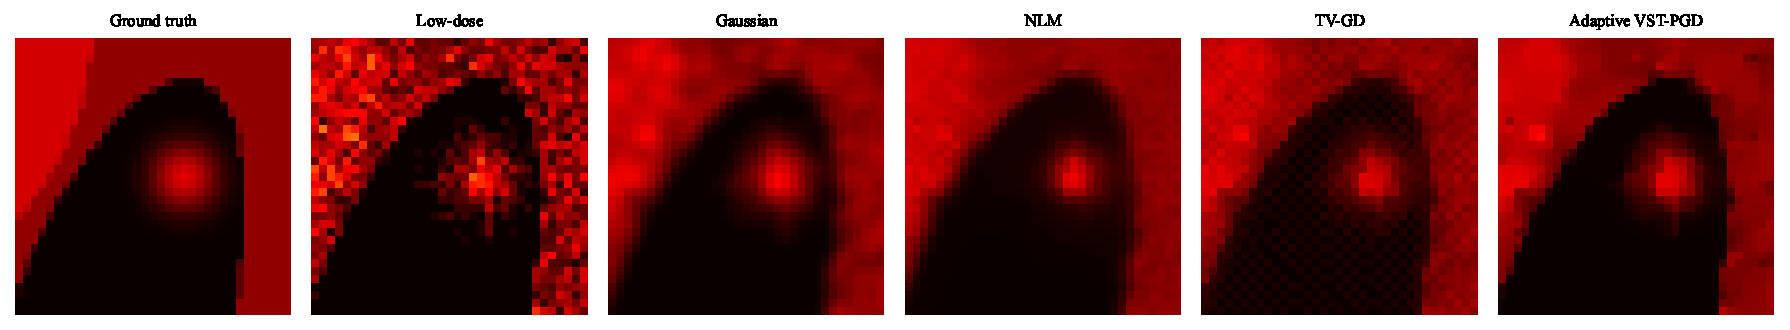
\includegraphics[width=.94\textwidth]{zoom_in.pdf}
\caption{Hot-lesion region used for local edge and shape assessment.}
\label{fig:zoom}
\end{figure}
\begin{figure}[tbp]
\centering
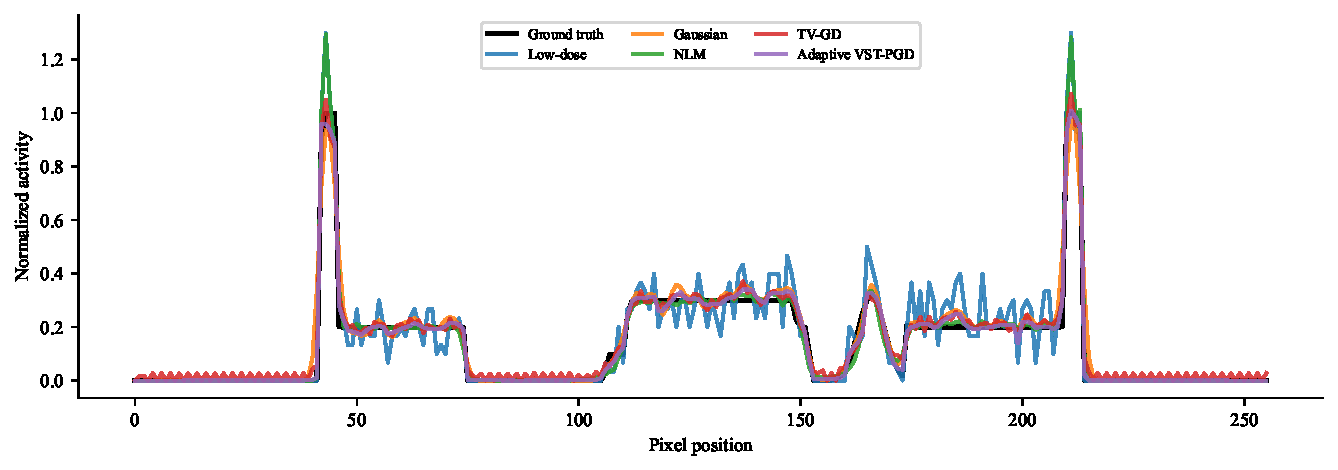
\includegraphics[width=.84\textwidth]{line_profile.pdf}
\caption{Horizontal activity profile through image row 102.}
\label{fig:profile}
\end{figure}

\subsection{Convergence Analysis}
Figure~\ref{fig:conv} reports the objective value and iterate-wise RE at 25\% dose. Spectral-step backtracking reached the stopping tolerance in \ProposedIterFifty{} and \ProposedIterTwentyFive{} iterations at 50\% and 25\% dose, respectively; the 10\% case used all \ProposedIterTen{} iterations, reflecting more difficult optimization under sparse counts.
\begin{figure}[tbp]
\centering
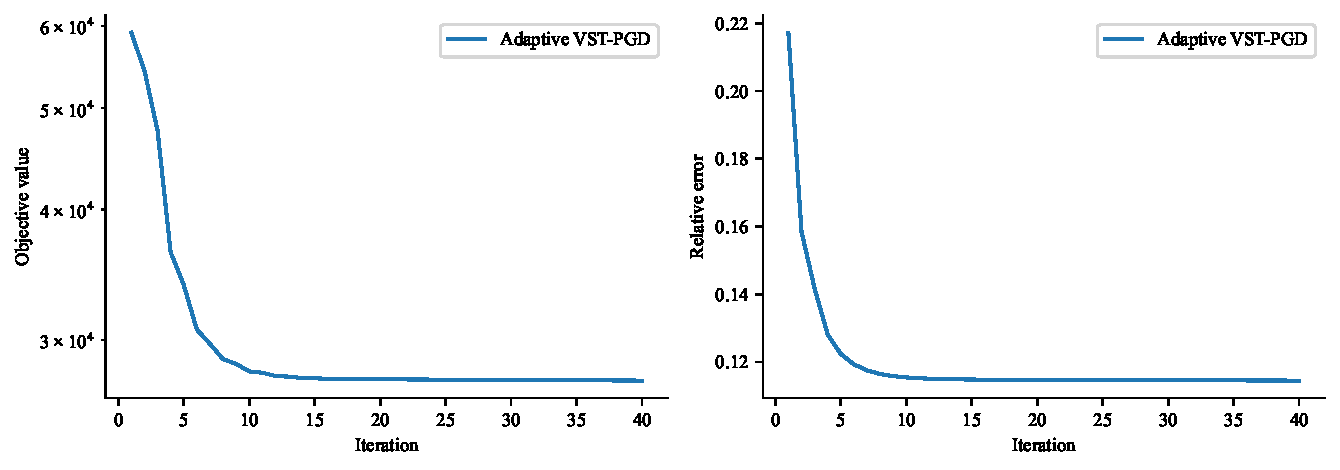
\includegraphics[width=.84\textwidth]{convergence_curves.pdf}
\caption{Measured Adaptive VST-PGD convergence history at 25\% dose.}
\label{fig:conv}
\end{figure}

\subsection{Ablation Study}
\begin{table}[tbp]
\centering
\caption{Ablation study at 25\% dose.}
\label{tab:ablation}
\setlength{\tabcolsep}{3pt}
\begin{tabular}{@{}lrrrrrrr@{}}\toprule
Variant & PSNR & SSIM & RMSE & RE & EPI & Time (s) & Iter.\\ \midrule
No Anscombe & 29.10 & 0.796 & 0.0351 & 0.145 & 0.968 & 0.0428 & 22 \\
No adaptive weight & 30.91 & 0.902 & 0.0285 & 0.117 & 0.983 & 0.2728 & 140 \\
Fixed-step PGD & 31.95 & 0.929 & 0.0253 & 0.104 & 0.988 & 0.6544 & 140 \\
Complete method & 31.49 & 0.899 & 0.0266 & 0.110 & 0.985 & 0.0791 & 40 \\
\bottomrule\end{tabular}
\end{table}
Removing the Anscombe transform caused the largest PSNR loss. Replacing the adaptive weight with uniform weighting reduced PSNR by \AdaptiveWeightPSNRLoss{} dB. Fixed-step PGD attained \FixedStepPSNR{} dB after \FixedStepIterations{} iterations, slightly above the early-stopped complete solver, but required \FixedStepRuntimeRatio{} times its runtime. The spectral step therefore improved practical convergence speed in this configuration rather than the best finite-budget PSNR.
\begin{figure}[tbp]
\centering
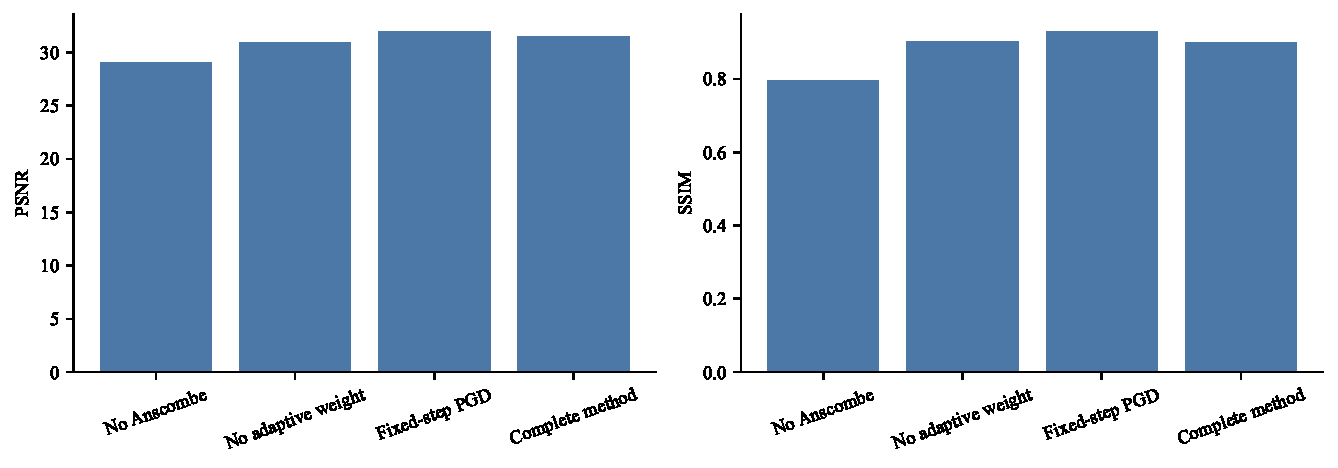
\includegraphics[width=.82\textwidth]{ablation_bars.pdf}
\caption{Ablation results at 25\% dose.}
\label{fig:ablation}
\end{figure}

\subsection{Parameter Sensitivity Analysis}
The grid in Fig.~\ref{fig:sensitivity} contains a broad high-PSNR region for $\lambda_1\in[1.6,2.0]$ and $\lambda_2\in[0.35,0.7]$. The best tested pair, $(\lambda_1,\lambda_2)=(\BestLambdaOne,\BestLambdaTwo)$, attained \BestSensitivityPSNR{} dB. Because this pair was selected on the evaluation phantom, an independent validation set would be required for clinical parameter selection.
\begin{figure}[tbp]
\centering
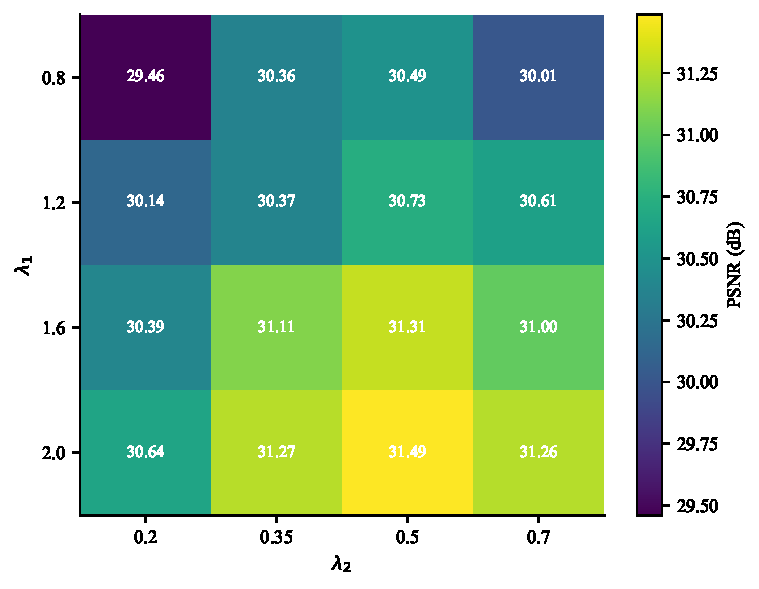
\includegraphics[width=.60\textwidth]{parameter_heatmap.pdf}
\caption{PSNR sensitivity to regularization parameters at 25\% dose.}
\label{fig:sensitivity}
\end{figure}

\section{Conclusion}
This study introduced Adaptive VST-PGD, a transparent low-dose PET preprocessing pipeline that combines Poisson variance stabilization, spatially adaptive first- and second-order regularization, and projected spectral-gradient optimization. Across three simulated dose levels, the method achieved the highest PSNR and competitive edge preservation, while NLM produced higher SSIM. Ablation results identified variance stabilization as the dominant component and confirmed a measurable contribution from adaptive weighting.

The numerical model omits scatter, random events, attenuation, resolution loss, reconstruction-induced correlation, and heterogeneous clinical anatomy. Periodic boundary operators may also introduce border interactions. Future work should evaluate reflective operators, the exact unbiased Anscombe inverse, direct Poisson-likelihood optimization, accelerated solvers, automated parameter selection, and lesion-level task metrics. Validation should progress from multiple digital phantoms to physical phantoms and ethically approved patient cohorts before clinical conclusions are drawn.

\bibliographystyle{unsrtnat}
\bibliography{references}
\end{document}
